Consider a set $\set{1,2,...,n}$ of $n$ distinct elements. Then we define a \textit{permutation} of $\set{1,2,...,n}$ as a bijection 
\[
	f: \set{1,2,...,n}\to \set{1,2,...,n}
\]
\begin{definition}
	The \textbf{symmetric group} $S_n$ is a set containing all such permutations of a set $\set{1,2,...,n}$.
\end{definition}
	In cycle notation we commonly see permutations of $S_n$ as (12),(23), etc. For our purposes, we'll each element will appear as an ordered list. That is,
	\begin{equation*}
		f(1)f(2)f(3)f(4) = (12) 
	\end{equation*}
	where $f(1) = 2$, $f(2)=1$, and $f(3)=3,f(4)=4$.
\begin{proposition}
	Let $S_n$ denote the set of all permutations of the set $\set{1,2,...,n}$. Then
	\begin{equation*}
		|S_n| =  n!
	\end{equation*}
\end{proposition}
\begin{proof}
	By definition, a permutation is a bijection
	\[
		f: \set{1,2,...,n}\to \set{1,2,...,n}
	\]
	We construct a bijection by specifying the values of $f(1),f(2),...,f(n)$ sequentially. There are $n$ possible choices for $f(1)$. Once $f(1)$ is chosen, by way of injectivity, any subsequent selection must have $n-k$ possible choices for $f(k+1)$, and for the final selection of $f(n)$ there exists exactly one element to choose from. Then, by the multiplication rule, the total number of such sequences of choices is 
	\begin{equation*}
		n\cdot(n-1)\cdot(n-2)\cdots = n!
	\end{equation*}
	Thus, $|S_n| = n!$.
\end{proof}
\begin{eg}
	Take a triangle $D_n$ does though, with 3 distinct vertices, each labeled 1,2,3 respectively. The symmetric group $S_3$ of all permutations of the triangle will have $3!$ total permutations.
	\begin{center}
		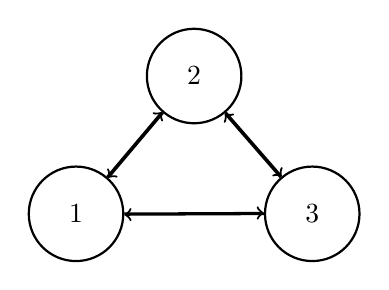
\begin{tikzpicture}[scale=.5,
			every node/.style={circle, draw, thick, minimum size=1.2cm},
			arrow/.style={->, thick}
			]
			
			% Nodes
			\node (1) at (0,0) {1};
			\node (3) at (6,0) {3};
			\node (2) at (3,3.5) {2};
			
			% Between 1 and 2
			\draw[arrow] ([xshift=-2pt,yshift=2pt]1) -- ([xshift=-2pt,yshift=2pt]2);
			\draw[arrow] ([xshift=2pt,yshift=-2pt]2) -- ([xshift=2pt,yshift=-2pt]1);
			
			% Between 2 and 3
			\draw[arrow] ([xshift=2pt,yshift=2pt]2) -- ([xshift=2pt,yshift=2pt]3);
			\draw[arrow] ([xshift=-2pt,yshift=-2pt]3) -- ([xshift=-2pt,yshift=-2pt]2);
			
			% Between 1 and 3
			\draw[arrow] ([yshift=3pt]1) -- ([yshift=3pt]3);
			\draw[arrow] ([yshift=-3pt]3) -- ([yshift=-3pt]1);
		\end{tikzpicture}
	\end{center}
\end{eg}
\begin{eg}
	Take a 52 card deck with no jokers. Shuffle the deck randomly. The total number of possible permutations of the deck is exactly 52!. 
\end{eg}
Up to this point, we have considered permutations of all $n$ elements.
We now ask how many permutations can be formed using only $k$ of the $n$
distinct elements. Rather than permuting all $n$ distinct elements, we may instead consider
permutations that involve only $k$ elements of the set.
\begin{definition}[Partial Permutation]
	The number of ways to choose and order $k$ elements from $n$ is 
	\begin{equation}
		P(n,k) = \frac{n!}{(n-k)!}
	\end{equation}
\end{definition}
\begin{eg}
	Consider a race of 10 total individuals. Determine the possible outcomes for the top 3 finishers. By the multiplication principle, we have $10\cdot 9\cdot 8$ selections for 3 stages, so we can write it as 
	\begin{equation*}
		\frac{10!}{(10-3)!} = \frac{(10)(9)(8)(7)\cdots(1)}{(7)\cdots(1)} = (10)(9)(8)
	\end{equation*}
\end{eg}
